% This template was created by Ben Mitchell
% for Dr. Sheppard's AI class, CS 335/435, spring 08.

% For those who want to learn LaTeX, this is a decent place to start:
% http://en.wikibooks.org/wiki/LaTeX
% Note that the proper pronunciation is "la tek", not "lay teks".
%
% There are lots of latex tutorials and primers online; just be careful with
% google images.

\documentclass[12pt,letterpaper]{article}

\usepackage{amsmath, amsthm, graphicx, multicol}

\title{Reinforcement Learning: \\Using Value-Iteration and Q-Learning}
\author{Bill Davis \\ Johns Hopkins University}


\begin{document}

\maketitle

\begin{abstract}
The paper discusses two reinforcement learning techniques, Value-Iteration and Q-Learning. Both algorithms are implemented and tested on the problem of navigating a probabilistic racetrack. These algorithms are then compared to an entropy based decision tree.
\end{abstract}

\section{Introduction}
Reinforcement learning is a way in which we can teach an agent to answer the question, "What Should I do?" That is, given a certain situation, and a set of possible actions, an agent needs to be able to select the appropriate action, avoiding actions which will not advance the agent toward its goals. In order for an agent to be able to intelligently learn which actions to take, given every possible state it might find itself in, reinforcement learning algorithms can be used to teach an agent proper behavior. 

Reinforcement learning is different from supervised learning techniques like decision trees or supervised learning algorithms, the instructor must already know the correct action for the agent to take. Those algorithms are designed to impart that knowledge upon the agent. Instead, reinforcement learning is a form of dynamic programming, that requires no other stimulus then a reward function. This reward function can be extremely simple, perhaps rewarding an agent for entering a certain square and ignoring it at other times. Then agent will attempt to learn the sequence of actions that can maximize the reward an agent will receive, or alternatively minimize the cost an agent will occur.  The dynamic programming takes place in the tables the agent will maintain while learning what the best action is to take, given the actions that it knows about so far. 

Reinforcement learning can also be successful even in situations where there is significant uncertainty regarding the actions that the agent can take. For example the agent may be unable to take actions that it would like to take, or alternatively may create an error when taking them. A good example is a moving robot. Due to sensor and motor error the robot may take an action to accelerate by 1 foot per second squared, which may actually correlate to a 1.5 foot per second acceleration. Being able to anticipate errors and account for them is a desirable trait of any intelligent agent, especially when an out of control robot may pose a hazard. Both Value-Iteration and Q-Learning allow for agents to take the best action in the face of this uncertainty, and arrive at maximum reward. 

The hypothesis of this paper is that Value-Iteration and Q-Learning will both generate the same solutions to the input problems, with Q-Learning taking longer to do so. The decision tree trained on the output of these learning algorithms will not perform as well as the algorithms themselves, however it will be more efficient in that the space required to store the decision tree will be significantly less then the full reinforcement learning tables.  

\section{Reinforcement Learning}
This paper considers two reinforcement learning algorithms. They are similar in many respects but they contain a few, key differences. 

\subsection{Value-Iteration}
Value-Iteration is based upon the concept of utility. 
\begin{quote}
Roughly speaking, the utility of a state if the expected utility of the state sequences that might follow. 
\end{quote}
As we can see of this definition of utility, the main job of Value-Iteration is to compute this expected utility. It does this through successive sweeps through the state and action space, updating utilities. Value-Iteration is based upon the Bellman Equation which is defined as 
\[
U(s) = R(s)+\gamma max_{a} \sum T(s,a,s')U(s')
\]
where R(s) is the reward at state s, and T(s,a,s') is the transition probability of moving from state s using action a to state s' \cite{aima}. This brings up the principal deficiency of the Value-Iteration algorithm. It requires that the T function is known, and that we have a model for the state action space. This extra information may not necessarily be known beforehand. And in face Q-Learning is capable of learning state, action sequences without knowing the model for the space a priori. 

Value-Iteration is able to converge to a solution to the Bellman Equation. It requires a table be maintained for the entire state and action space, Q-Learning has the same requirement. This can obviously be prohibitive for large state spaces. 

\subsection{Q-Learning}
Q-Learning is a learning method which learns action-value pairs as opposed to the utility learning of Value-Iteration. It is also an off-policy learning algorithm. This means that Q-Learning is able to learn a policy while effectively trying out different ones \cite{riai}. This is as opposed to an on-policy algorithm like SARSA which can only learn about the greedy policy while exploring the greedy policy. 

By having Q-Learning only reinforce action-value pairs, a probabilistic model is not required before the algorithm can be run. Q-Learning can also be used on-line and will return answer with increasing accuracy as the algorithm runs. The Q-Value is defined as 
\[
Q(a,s) = R(s) + \gamma \sum_{a}T(s,a,s')max_{a'}Q(a',s')
\]

\subsection{Entropy Decision Trees}
A entropy based decision tree was also developed to navigate the race track. For each course a training set was generated, which was then use to create a decision tree. The decision tree acted on state space and returned an action, either accelerate or not. It was hoped that the decision tree would be able to generalize about the state space and require less data encoding then the entire state space table.  

\section{Algorithms and Experimental Methods}
For these experiments three data sets were used, with progressively more difficult. These are identified as the L-Track, O-Track and R-Track, where each track appears like the letter identifying it. Each algorithm was run on each track, with the intent to find the least cost path from a start node to a finish node. At each node the agent can either accelerate or not, in either positively negatively, in both the x and y directions. Each agent was also tested on two crash rules on each track. The first rule states that the agents velocity becomes zero on a crash. The other rule is that the velocity is set to zero and the agent is reset to a starting position after a crash, obviously this second rule is much stricter about crashes then the first. 

Each algorithm was run for multiple iterations. At the end of each iteration, a number of simulated cars were driven from the start node to finish node. If they failed to complete the trip in under 100 moves the trip was declared a failure. Each algorithm was run until it appeared to converge on a least cost solution to the problem. 

Once the Value-Iteration algorithm has converged on a solution, the state space was written out as training data to be used to construct a decision tree. This decision tree was constructed with the gain ratio adjustment, but without pruning. A number of simulated cars was then driven according to actions selected by the decision tree. 

Both algorithms contain a learning parameter $\gamma$, this was set to 0.9 in the Value-Iteration algorithm and to 0.5 for Q-Learning. Both of these parameters were chosen to minimize runtime while still arriving at optimal solutions. The Q-Learning parameter was especially difficult to tune. 

Because this is a least cost-problem rather then a max-reward problem both reinforcement learning algorithms required slight modification. This was to select the least cost path as opposed to the max reward when making decisions. The exploration technique used for Q-Learning also required slight modification; this is discussed in the discussion section. These were the only modifications that were required. 

\section{Results}
The results of the multiple experiments are listed below. 


Table-1 shows the final result of all algorithms run over all race tracks. The value shown is the least cost path as determined by the algorithm. Each race track has two runs, one where the velocity is merely set to zero upon crash and another where the velocity is set to zero and the car is reset to a starting position. 

% Table generated by Excel2LaTeX from sheet 'Sheet1'
\begin{table}[h]
\begin{tabular}{|r|r|r|r|}
\hline
     Track & Value Iteration & Q-Learning & Decision Tree \\
\hline
   L-Track &      12.82 &      16.37 &       12.8 \\

L-Track With Reset &      14.44 &      16.02 &      14.61 \\

   O-Track &      25.01 &      26.82 &      24.72 \\

O-Track With Reset &      31.11 &      34.11 &       31.7 \\

   R-Track &       26.8 &      29.31 &      26.56 \\

R-Track With Reset &      33.43 &      36.95 &      34.25 \\
\hline
\end{tabular}  

\caption{Results for all algorithms and all race tracks. }
\end{table}

Table-2 shows the number of node evaluations required before the algorithm achieved converged on a solution. These numbers are only an estimate in the case of Q-Learning because for that algorithm no precise computation was done to determine precise convergence. The numbers are presented as Nodes (Iterations) Iterations are different between Value-Iteration and Q-Learning, but are node evaluations are the same. In Value-Iteration an iteration is considered as one entire sweep over the state space. In Q-Learning an iteration is a path that goes from start node to finish node.

% Table generated by Excel2LaTeX from sheet 'Sheet1'
\begin{table}[h]
% Table generated by Excel2LaTeX from sheet 'Sheet1'
\begin{tabular}{|r|r|r|}
\hline
           & Value Iteration & Q-Learning \\
\hline
   L-Track & 212960 (10) & 2074186 (11000) \\

L-Track With Reset & 212960 (10) & 2965015 (5750) \\

   O-Track & 612260 (22) & 4201873 (18500) \\

O-Track With Reset & 745360 (27) & 5831460 (6250) \\

   R-Track & 886325 (24) & 5995253 (17750) \\

R-Track With Reset & 1063590 (29) & 8159443 (2250) \\
\hline
\end{tabular}  
 
\caption{Node evaluations (Iterations) for Q-Learning and Value Iteration}
\end{table}



Figure-1 demonstrates the convergence of Q-Learning over multiple iterations for a single track, in this case the O-Track without reset. This chart shows that after an initial uncertain period, Q-Learning eventually settles down close to an optimal solution. 

\begin{figure}
\begin{center}
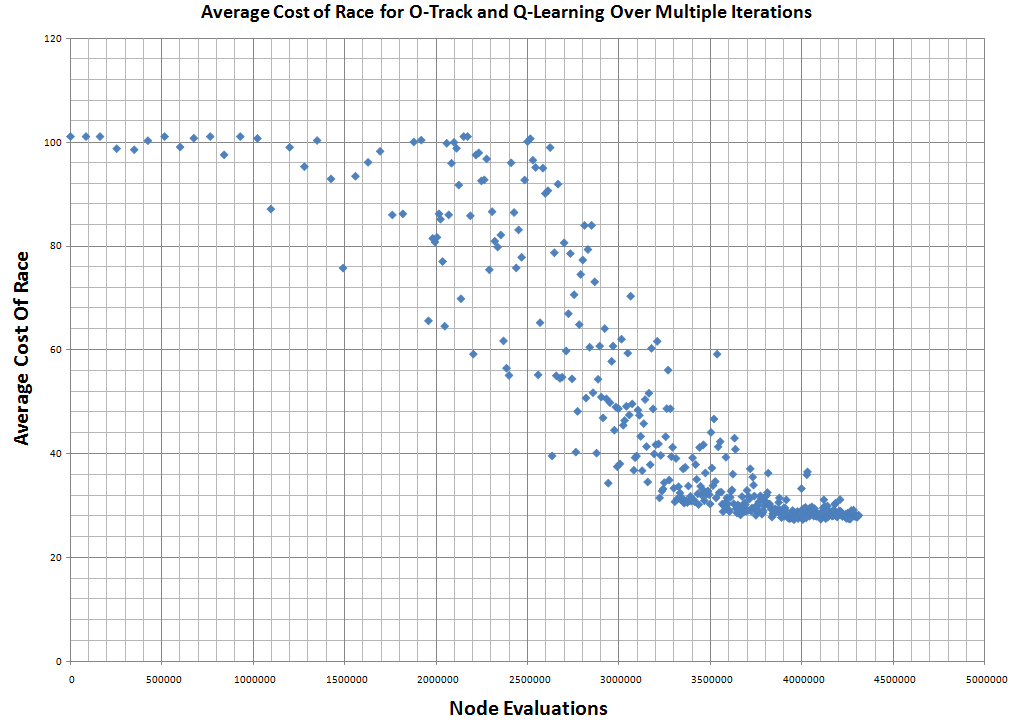
\includegraphics[width=6.5in]{Q-Learning.png}
\end{center}
\caption{Shows the covergence of Q-Learning over multiple node evaluations}
\label{qlearning}
\end{figure}



\begin{table}[h]
% Table generated by Excel2LaTeX from sheet 'Sheet1'
\begin{tabular}{rrrrr}

X Multiplier & Y Multiplier & Reset Condition &    Average & Node Count \\
\hline
         1 &          1 &        Off &       25.1 &      63771 \\

         1 &          1 &         On &      32.69 &      65608 \\

         1 &          2 &        Off &      90.48 &      31900 \\

         1 &          2 &         On &       65.5 &      34981 \\

         1 &          3 &        Off &      92.26 &      15284 \\

         1 &          3 &         On &      98.13 &      23459 \\

         1 &          4 &        Off &      95.98 &      11842 \\

         1 &          4 &         On &      84.32 &      17612 \\

         2 &          1 &        Off &      52.51 &      33843 \\

         2 &          1 &         On &      51.39 &      34310 \\

         2 &          2 &        Off &      66.42 &      16642 \\

         2 &          2 &         On &      44.42 &      18618 \\

         2 &          3 &        Off &      59.61 &       7827 \\

         2 &          3 &         On &      91.03 &      12613 \\

         2 &          4 &        Off &      78.54 &       6292 \\

         2 &          4 &         On &      77.49 &       9416 \\

         3 &          1 &        Off &      85.35 &      22794 \\

         3 &          1 &         On &      83.59 &      23020 \\

         3 &          2 &        Off &      98.82 &      12399 \\

         3 &          2 &         On &      69.37 &      12374 \\

         3 &          3 &        Off &      73.39 &       5199 \\

         3 &          3 &         On &         99 &       8511 \\

         3 &          4 &        Off &      93.94 &       4199 \\

         3 &          4 &         On &      77.86 &       6572 \\

\end{tabular}  
\caption{Differing quantization's of the position state space and the effects on the decision tree algorithm. The effect of the X and Y multiplier was to reduce the apparent number of possible x and y positions for the decision tree to process. All experiments for this chart were run on the O-Track}

\end{table}

Table-3 shows the effects of further reducing the state space of the O-Track. When generating the training data the X and Y positions were divided by the multiplier. The effect of this was to create a blockier space, so that the decision tree was not required to learn about every possible board position. When the average cost was computed the maximum was determined to be 100, meaning that at 100 iterations the agent effectively gives up. Therefore values close to a hundred correlate to a failure of the decision tree to navigate the car to the finish line. 



\section{Discussion}
All of the algorithms evaluated were able, given enough processing time, to generate good solutions to the problem of least cost paths between start and finish squares on the race track. Value-Iteration was able to generate the least average path cost. This is not surprising as Value-Iteration requires that a model of the problem be developed before evaluation. Q-Learning, which is capable of inferring the model given enough samples, required longer to evaluate and produced slightly higher average cost paths. The decision tree, trained on the value-iteration data, was able to almost duplicate the results of Value-Iteration. More on these results will be discussed below. 

\subsection{Value Iteration}
Value Iteration was the most highest performing of the algorithms. It was able, in the fewest number of node evaluations to generate the paths with the least cost. This was true for all race tracks and all restart conditions. The run-time of the algorithm was dependent not only upon the size of the sample space, but also depended upon the complexity of the scenario. For these tests, for example, learning how to operate under the restart condition took more node evaluations for both the O-track and the R-track. The runtimes were the same for the L-track, but this was likely due to the simplicity of that data set. 

This algorithm showed some unexpected behavior when minimizing the cost function. For example on the L-track the algorithm correctly computed that crashing into the wall before the finish was the fastest manner to get to the finish line. This was with the reset condition off, of course. The results when using the reset condition were more conservative in nature, and always took longer. The agent weighed going faster against the probability of crashing. The training data that was generated when the reset condition was on was also more effective when being used to train the decision tree. 

\subsection{Q-Learning}
Q-Learning is slightly more complicated then Value-Iteration. It required significantly, sometimes ten times as many, node evaluations as Value-Iteration, before achieving results which were not quite as low as the Value-Iteration results. One of the more interesting results was in the number of iterations required for a solution. This was lower in the case of the Tracks with the reset condition in place. This is counter-intuitive because this is the more difficult case, but can be explained because the number of node-evaluations was still higher. This was because an iteration in the Q-Learning case was defined as moving the agent from the start condition to the finish line. This required the agent to explore significantly more of the state space before completing a single iteration when the reset condition was on. 

\subsubsection*{Q-Learning Exploration}
Q-Learning is a more complicated algorithm because it requires an initial policy in order to properly explore the space, before any of the Q-values can be generated \cite{wiki}. For these experiments the a Boltzmann equation was used. This equation 
\[
B(a)=\frac{e^{Q(s,a)/k}}{\displaystyle\sum_{a'\in Q(s)}e^{Q(s,a')}}
\]
The probability that a specific action is chosen is proportional to it boltzmann value. This equation uses a temperature parameter $k$ which is slowly decreased over the course of the runtime of the algorithm. The values used for this experiment was an initial temperature parameter of 100.0, which is decreased by 0.00005 for every evaluation until the temperature equals zero. The effect of this is that the selection of actions during the initial runtime of the algorithm is effectively random, and slowly changes policy until the action that is the selected is entirely based upon the Q-Value of the state the agent is in. These parameters were tuned to give good run-times for these experiments. 

The net effect of this exploration function is that there is an initial period of time when results generated from Q-Learning are no better then a random walk. Then there is a long period of time with sporadic results, some very good, others very bad, as the agent explores the possible solutions. Then when the temperature has dropped enough, the agent enters into a convergent state where it will always produce good results. 

\subsection{Function Approximation}
For these experiments a decision tree was used a function approximator. Several experiments were run on the state space in order to determine an optimal training set. 

Given the output of the Value-Iteration algorithm the entropy based decision tree was capable of reproducing the results generated by the value-iteration algorithm. Unfortunately it required an excessive number of nodes to do this. Attempts were made to reduce the statespace and further quantize the training data. These were somewhat effective, although any attempt to reduce the training data resulted in a loss of performance. There was some success, as can be shown in table-3. By quantizing the O-Track into 2 by 2 squares, effectively cutting the state space by 4, a 4 times reduction in the number of nodes in the decision tree was produced. The resulting decision tree was still able to navigate the O-Track with both the reset condition on and off, although the average cost was twice that of average cost produced by the Value-Iteration algorithm.  

Overall this is somewhat disappointing. It was expected that the trained decision tree would do a better job at generalizing about the state space. It is possible that more intelligent mechanisms of chunking up the state space could result in the decision tree performing better, but these methods might be overkill when the chief benefit of decision trees is their simplicity. 

Another mechanism that we can identify, but didn't try, is that the training set used when the reset condition is on was more conservative then the other set, and performed better when the examples used in training were reduced. It might be possible to use this training set for both condition, reset on and off, to achieve better results. 

\section{Conclusion}
Value-Iteration is clearly the superior algorithm tested in these experiments. It was able to produce the lowest cost paths while examining the fewest nodes. Unfortunately Value-Iteration is not always appropriate in real-world situations, and requires that a probabilistic model be developed before the algorithm can be run. Q-Learning then is a good algorithm which improves upon these deficiencies. The answers that are obtained from Q-Learning in these experiments were not as good as Value-Iteration, however there were quite close given sufficient running time. This run-time was significantly longer then what was obtained in Value-Iteration and is likely highly dependent upon the problem being solved as well as the parameters selected to solve it. 

In this case a decision tree was also used for agent control. It was able to duplicate the solutions produced by Value-Iteration, but contained so many nodes to do so that there is no benefit to using the tree model over the reinforcement table. Attempts to reduce the number of nodes used in the tree by quantizing the state space were effective but resulted in a loss of performance of the resulting decision tree. 

\bibliographystyle{plain}
\bibliography{bill_davis_pa3}
\end{document}
